\documentclass{beamer}
% \documentclass[handout]{beamer}
% \setbeameroption{show notes}

\usecolortheme[named=blue]{structure}

\mode<presentation>
{
  \usetheme{Warsaw}
  \setbeamercovered{transparent}
}
\title
  [SemFix: Program Repair via Semantic Analysis]
  {SemFix:~Program~Repair~via~Semantic~Analysis}
\author[DeMarco]{Favio~DeMarco}
\institute[U.B.A. - INRIA]{Universidad de Buenos Aires - INRIA}
\date[08/28/2013]{August 28th, 2013}
\subject{Computational Sciences}

% Programming today is a race between software engineers striving to build bigger and better idiot-proof programs, and the Universe trying to produce bigger and better idiots. So far, the Universe is winning.
% Rick Cook, The Wizardry Compiled

\begin{document}

\frame
  {
    \titlepage
  }
%-----------------------------------------------------------------------------80
  \section*{Outline}
%-----------------------------------------------------------------------------80
  \frame
  {
    \frametitle{Outline of Topics}

    \tableofcontents
  }

{
\usebackgroundtemplate{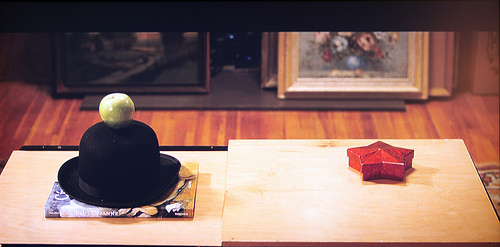
\includegraphics[width=\paperwidth]{500daysofsummer}}%
  \frame
  {
    \frametitle{State of the art}
  }
}

  \frame
  {
    \frametitle{Semfix}
	\Huge Let there be boxes!
	\note{An automated repair method based on symbolic execution, constraint solving and program synthesis. Semfix tries to fix a bug using symbolic execution, an SMT solver and program synthesis.}
  }

\end{document}
